\documentclass[a4paper]{jpconf}
\usepackage{layouts}[2001/04/29]

\def\mychapterstyle{default}
\def\mypagestyle{headings}
\def\revision{}
\usepackage{fancyvrb}			% Allow \verbatim et al. in footnotes
\usepackage{graphicx}			% To include graphics in pdf's (jpg, gif, png, etc)
\usepackage{booktabs}			% Better tables
\usepackage{tabulary}			% Support longer table cells
\usepackage[utf8]{inputenc}		% For UTF-8 support
\usepackage{xcolor}				% Allow for color (annotations)

%\geometry{landscape}			% Activate for rotated page geometry

%\usepackage[parfill]{parskip}	% Activate to begin paragraphs with an empty
								% line rather than an indent


\def\myauthor{Author}			% In case these were not included in metadata
\def\mytitle{Title}
\def\mykeywords{}
\def\mybibliostyle{plain}
\def\bibliocommand{}

\VerbatimFootnotes
\def\affiliation{Northastern University, USA. Princeton University, USA.}
\def\myauthor{Giulio Eulisse, Lassi Tuura, Peter Elmer}
\def\baseheaderlevel{2}
\def\mybibliostyle{apa}
\def\format{complete}
\def\latexxslt{jpsconf}
\def\latexheader{foo}
\def\mypagestyle{jpconf}
\def\mytitle{HEP C++ meets reality}


%
%	PDF Stuff
%

%\ifpdf							% Removed for XeLaTeX compatibility
%  \pdfoutput=1					% Removed for XeLaTeX compatibility
  \usepackage[
  	plainpages=false,
  	pdfpagelabels,
  	pdftitle={\mytitle},
  	pagebackref,
  	pdfauthor={\myauthor},
  	pdfkeywords={\mykeywords}
  	]{hyperref}
  \usepackage{memhfixc}
%\fi							% Removed for XeLaTeX compatibility


%
% Title Information
%

\ifx\subtitle\undefined
\else
	\addtodef{\mytitle}{}{ \\ \subtitle}
\fi

\ifx\affiliation\undefined
\else
%%	\addtodef{\myauthor}{}{ \\ \affiliation}
\fi

\ifx\address\undefined
\else
%%	\addtodef{\myauthor}{}{ \\ \address}
\fi

\ifx\phone\undefined
\else
	\addtodef{\myauthor}{}{ \\ \phone}
\fi

\ifx\email\undefined
\else
	\addtodef{\myauthor}{}{ \\ \email}
\fi

\ifx\web\undefined
	\else
		\addtodef{\myauthor}{}{ \\ \web}
\fi

\begin{document}
\title{\mytitle}
\author{\myauthor}


% Title
% Copyright Info
\setlength{\parindent}{0pt}

\ifx\mycopyright\undefined
\else
	\textcopyright{} \mycopyright
\fi

\revision

\setlength{\parindent}{1em}

%
% Main Content
%


% Layout settings
\setlength{\parindent}{1em}

\begin{abstract}
\label{abstract}
\addcontentsline{toc}{section}{Abstract}

In 2007 the CMS experiment first reported some initial findings on the impedance mismatch between HEP use of C++ and the current generation of compilers and CPUs. Since then we have continued our analysis of the CMS experiment code base, including the external packages we use. We have found that large amounts of C++ code has been written largely ignoring any physical reality of the resulting machine code and run time execution costs, including and especially software developed by experts. We report on a wide range issues affecting typical high energy physics code, in the form of coding pattern - impact - lesson - improvement.


\end{abstract}

\section{Mismatch between CPU and code}
\label{mismatchbetweencpuandcode}

When writing in C++ physicists have the tendency to think that the CPU will somehow be able to digest any code produced by the compiler. In particular we tend to think that memory operations have no latency, the memory structure is flat, branches are cheap and that the CPU is always able to find out what instruction to do next.
Reality is however much different.


While processor performances have evolved in exponentially, following the so called {\itshape Moore's law}~\cite{Moore:1998p325}, (dynamic) RAM memory has not kept up the pace with the result that its access has huge latency. The net result is that the faster processor the higher is the risk of  having it sitting idle waiting data or code coming from memory. This is commonly referred as the {\itshape Memory Wall}.


Well aware of  this, all the CPU vendors try to mitigate the problem in various ways. First of all, modern CPUs have a hierarchy of  so called {\itshape cache memories} which are small quantities of on chip RAM implemented using the much faster (but much more expensive) {\itshape static} RAM cells which act as intermediary between the slow main memory and the CPU. Moreover, various  way of predicting (~\cite{Smith:1998}, ~\cite{Uht:1997}) the program flow and mitigating the cost of pipeline stalls due to branches are used. In particular most of  mainstream CPUs implement a branch prediction unit that use branch history to predict whether or not a given branch will be executed. Finally, the {\itshape Memory Management Unit} (MMU) of a CPU is equipped with so called {\itshape Translation Lookaside Buffers} (TLBs) which assist the conversion between the virtual address space where a program run and the physical address space. While all this devices alleviate the cost of  memory access and push the memory wall forward, technological limitations make so that those resources are actually small and in general limited.


Just to give an example, a relatively new Core 2 Duo (tm) ~\cite{Core2Duo} processor from Intel has the specs show in \autoref{moderncpuspecs}:


\begin{table}[htbp]
\begin{minipage}{\linewidth}
\setlength{\tymax}{0.5\linewidth}
\centering
\small
\caption{Modern CPU specs}
\label{moderncpuspecs}
\begin{tabulary}{\linewidth}{@{}lc@{}} \\ \toprule 
\multicolumn{2}{c}{Core 2 Duo E8000 series} \\\midrule
L1 Instruction Cache Size (kB)&32kB \\
L1 Data Cache Size (kB)&32kB \\
L2 Unified Cache Size&6MB, shared by all cores \\
Number of 4kB pages entries in the TLB&128 \\

		\bottomrule
	\end{tabulary}
\end{minipage}
\end{table}

As time goes by and technology / economics permits those numbers obviously increase, but so far what we have is a few kilobytes of L1 caches and a few megabytes of L2/L3 cache. Moreover things get even more complicated ~\cite{Innocente:2009} due to the multi-core nature of latest generations of CPUs.


If we then look at some of the characteristics of CMS offline reconstruction software (CMSSW ~\cite{Jones:2006}) as shown in \autoref{cmssw}


\begin{table}[htbp]
\begin{minipage}{\linewidth}
\setlength{\tymax}{0.5\linewidth}
\centering
\small
\caption{CMSSW}
\label{cmssw}
\begin{tabulary}{\linewidth}{@{}lc@{}} \\ \toprule 
\multicolumn{2}{c}{Numbers for a representative workflow} \\\midrule
Size of a representative executable&200MB \\
Actual size of CODE sections&50MB \\
Average number of libraries loaded&500 \\
Number of symbols in one single executable&50K \\
Representative VSIZE for a run&1GB \\
Size of the event&2MB \\

		\bottomrule
	\end{tabulary}
\end{minipage}
\end{table}

we see a clear mismatch between what the hardware provides and the inherent dimensions in play of CMSSW. If on one side we talk about dozens of kilobytes for L1 caches and a few megabytes for the L2 ones, on the other side we are in the hundreds of megabytes of code size and, particularly peculiar for our software, is the vast amount of symbols and shared libraries. While these last item might not seem of too much importance to a first look, one has to think that due to the nature of dynamic code, symbol tables do have to be loaded into memory at execution time and every single library has to be loaded in a separate page, therefore increasing pressure on the ITLB. Moreover, as reported separately ~\cite{Elmer:2009} the overheads due to this large amount of symbols and libraries make the port to 64 bit architecture more difficult.


\section{Understanding the reasons for the mismatch}
\label{understandingthereasonsforthemismatch}

One first naive question is whether or not such an amount of code is actually needed. By instrumenting our software using gcov and checking the source code coverage of a single, but representative, workflow, we found out that only one third of the lines of code are actually executed for this one third, only half of it is actually executed more than once. The main problem is that the executed and non-executed parts of the code are actually mixed in and it's therefore very hard for the memory management system to separate them so that the {\itshape cold} parts are polluting the execution of {\itshape hot} ones.
This actually matches with our past work ~\cite{Tuura:2008p00019} where we identified high ITLB pressure as one of the problems for CMS software.
The reasons for this large amount of code are actually multiple, but they can be summarized in four major areas:


\begin{itemize}


\item naive programming mistakes

\item over-generic code \& bad packaging of features which should have been kept separate

\item C++ specific idiosyncrasies

\item the legitimate need for exceptions, debug statements and boundary conditions
\end{itemize}

Moreover a detailed split-up of the contents of our software (see fig. 1) shows how only half of the software size is due to \texttt{CODE} sections and that exceptions, string literals and symbols have a large contribution to the final size.


\begin{figure}
\caption{CMSSW linker sections}
\label{}
\begin{center}
\resizebox{350pt}{!}{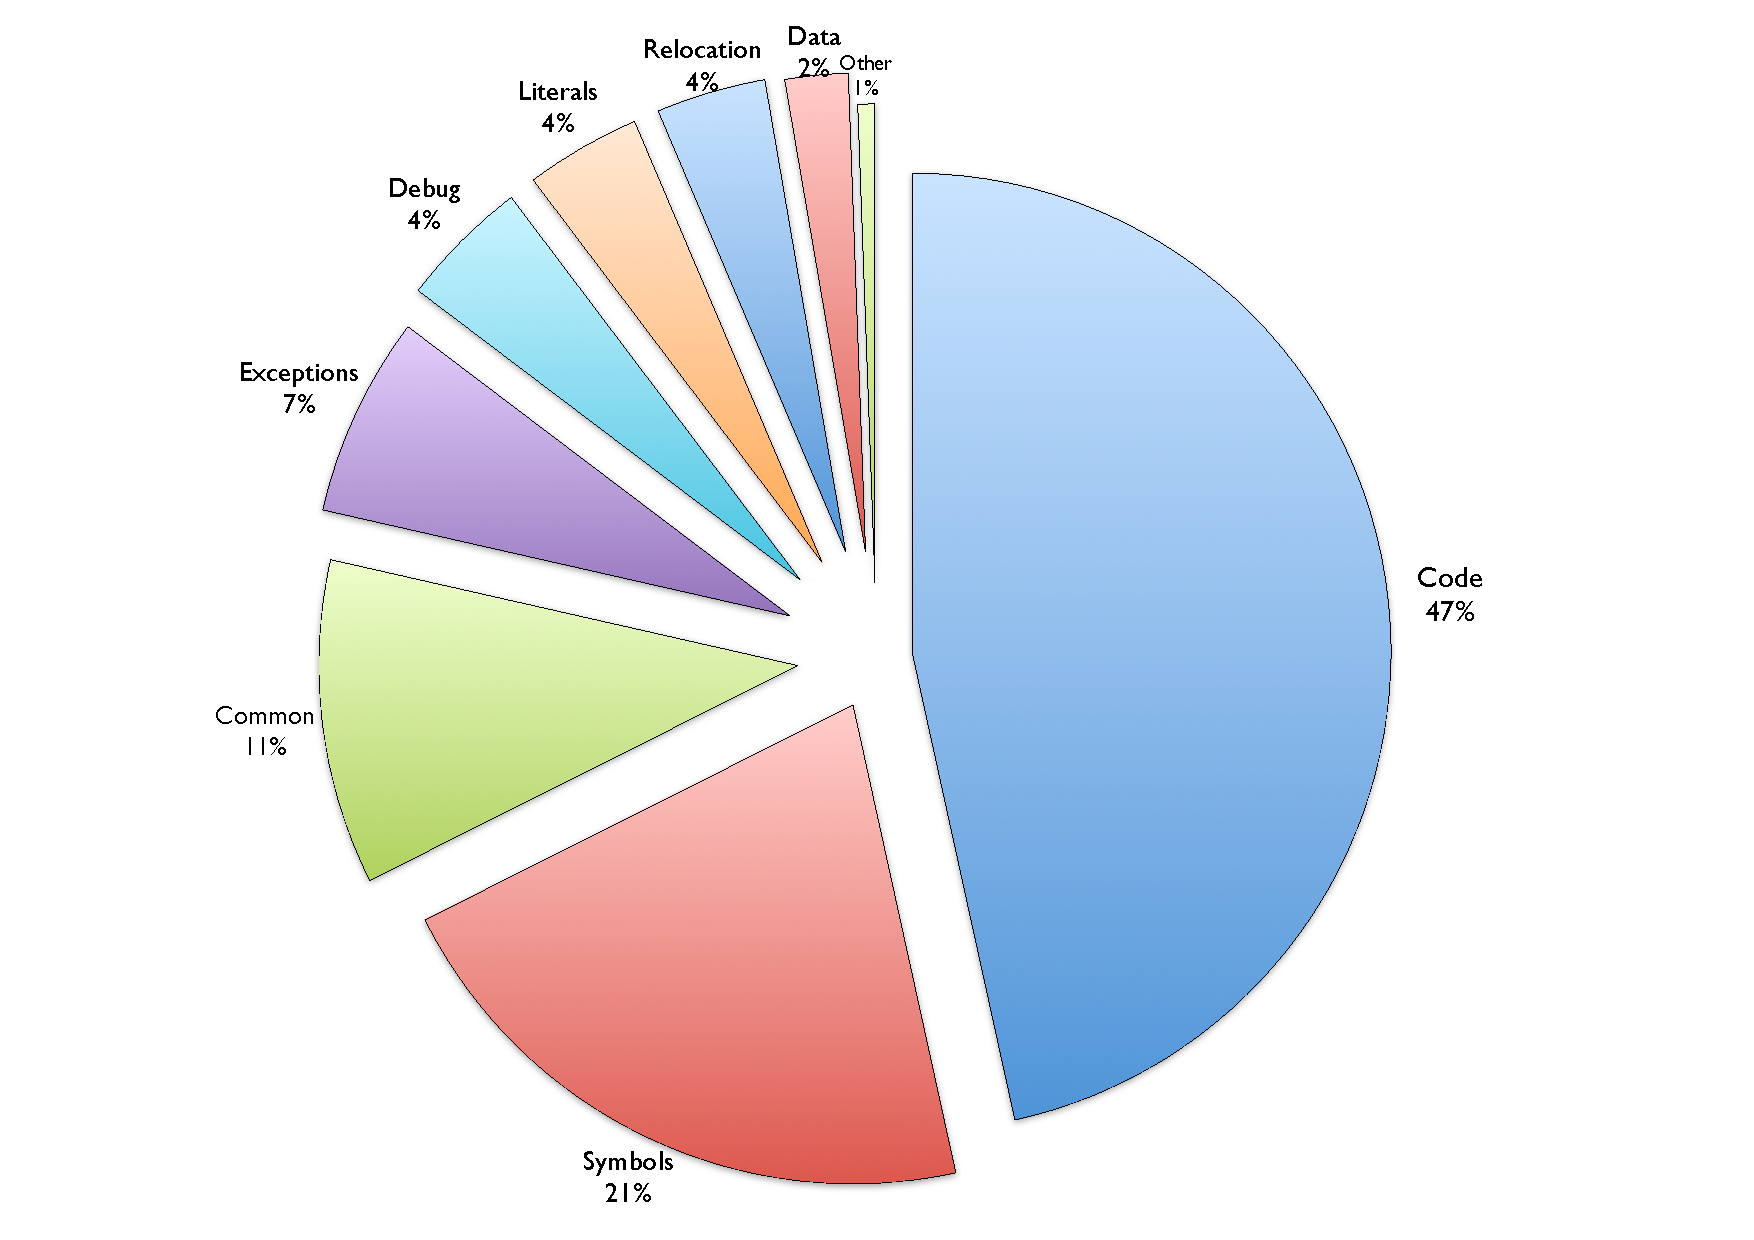
\includegraphics{cmssw-splitup.pdf}}
\end{center}
\end{figure}



Strong of this understanding and its support data we have started an effort to try to reduce the size of our executable, knowing that this would have had for sure a concrete impact in things like memory usage (since code is actually a rather large fraction of our memory footprint), but also with the hope that this reduction in code-size would have brought an improvement in performance by alleviating pressure off the CPU caches and TLBs.


One example was discovered while trying to understand why we had so much space devolved to symbol names. It turned out that the object persistency dictionary generator was mangling helper methods names with the file name of the source file where the actual method was defined, including the path relative to where the dictionary generator was getting launched. Changing directory to the actual location of the source file, before invoking genreflex and using a temporary, short, filename was enough to reduce by 9 MB the size use in the executable due to those symbols. This is a lampant example of how it's not only important write correct code, but that build procedures and packaging of the various software components has a non negligible impact on the produced code.


\subsection{Study of symbols size}
\label{studyofsymbolssize}

The simplest thing that we can do when trying is to try to plot the size of symbols and their size in a scattered plot like the one shown in figure 2.


\begin{figure}
\caption{}
\label{}
\begin{center}
\resizebox{250pt}{!}{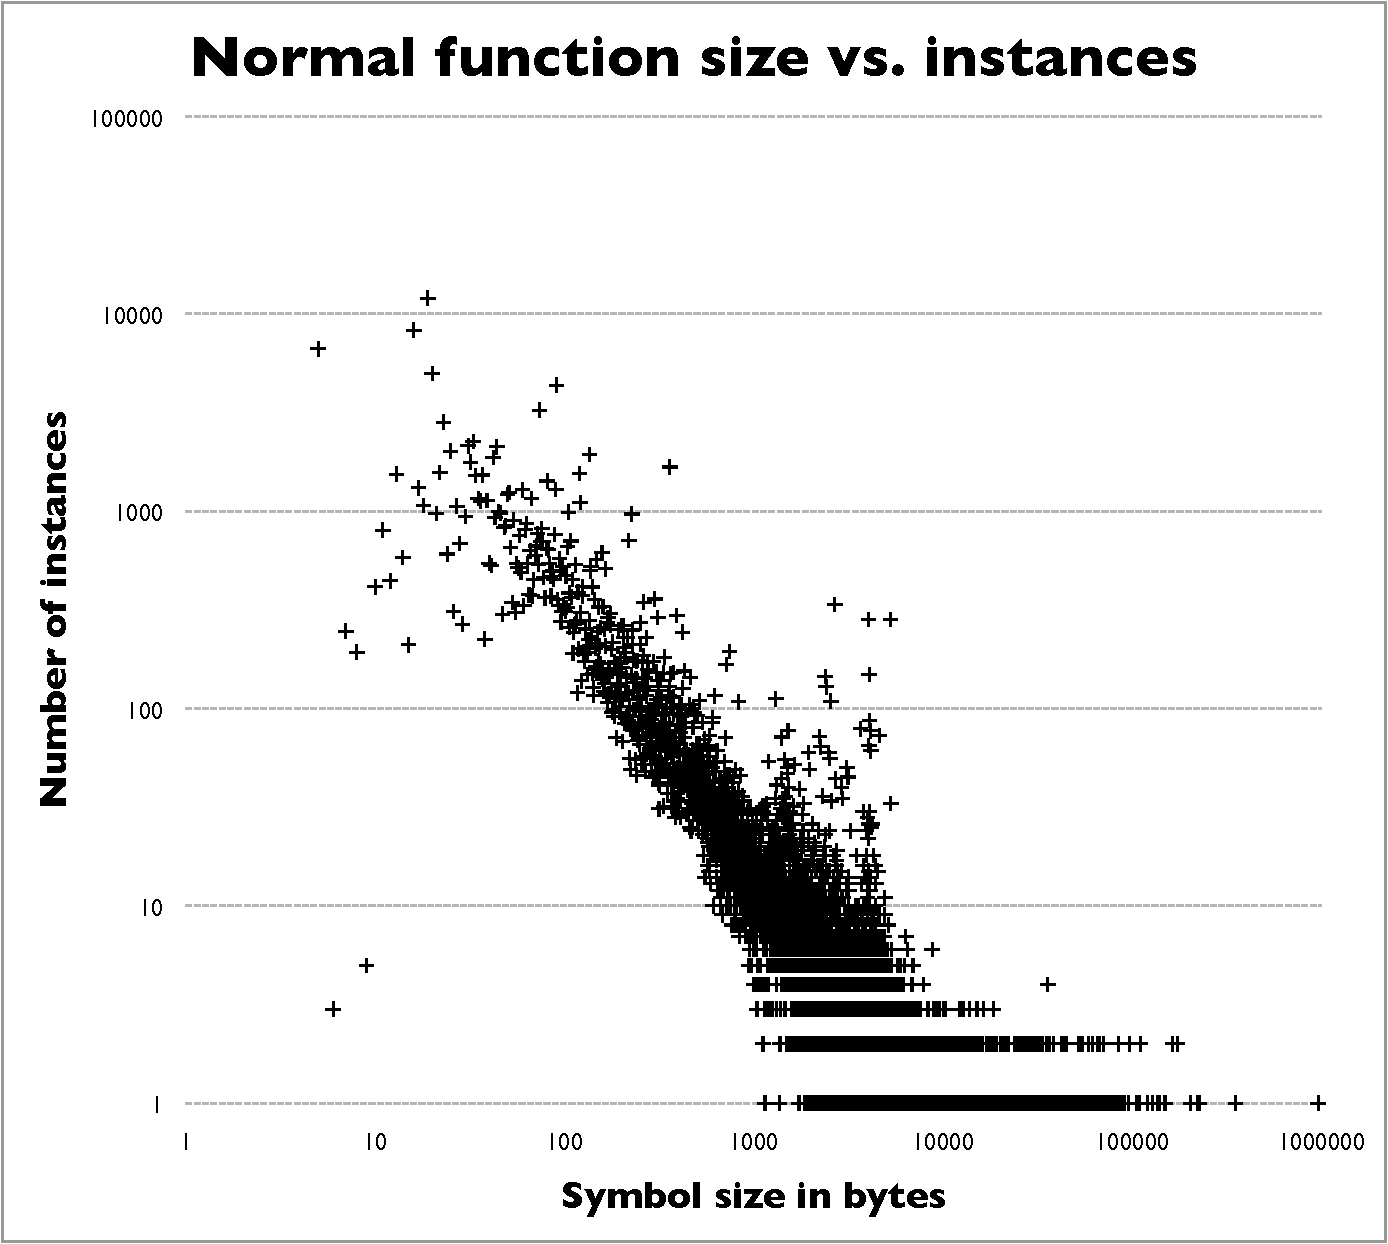
\includegraphics{Normalfunctionsizevsinstances.pdf}}
\end{center}
\end{figure}



This clearly shows that there are two different kind of issues:


\begin{itemize}


\item Symbols which are suspiciously large

\item Multiple symbols which suspiciously have all the same size
\end{itemize}

In the first case we found the problem laying in some common coding patterns that were forcing the compiler to inline too much code. In particular we found that having missing, either because of template classes or because of laziness, out-of-line destructors were responsible for a number of cases in which the code size exploded with no apparent reason. We have found that this reaches pathological levels in the case exceptions have been thrown and gcc find himself unable to detect which exit paths are actually the same and is actually forced to delete temporary objects (therefore inlining the constructor) on every separate exit path.


The second case is instead peculiar for template classes and in particular it results in pathological (aggregate) symbol sizes when non template invariant code is left inside templated classes. In this case gcc is unable to recognize the code as common (even in the case of simple types like int or unsigned int) and produces duplicate copies of the same code. Optimizing and making sure this does not happen is of particular interest for CMS, since due to CMSSW design there are a number of template classes (especially smart pointers and custom collections used for persistency) which get templated over a large number ( O(400) ) of {\itshape physics event objects}. Of course the worst case scenario is when both things happens and we have actually found parts of our code base where this was the case.


\section{Using perfmon2 to profile big C++ code-bases}
\label{usingperfmon2toprofilebigccode-bases}

{\itshape Perfmon2}~\cite{Eranian:2006p467} is a low level profiler for Linux, taking advantage of modern processors self-inspection capabilities ~\cite{Anderson:1997}. In particular it is able to produce a statistical profile of which part of a program used / abused more a given CPU resource (instruction cache, BPU, TLBs) or even just where the actual time was spent.
The problem is that in order to have a low overhead on the profiled application the implementation of perfmon2 only provides flat reports, where the stack trace information is lost. In poor words one gets to know that a given function is causing a lot of instruction cache misses, but no information about what called that function is given. The net result, at least for large software like CMS one, is that a large fraction of the cost reported comes from usual suspects (like malloc, free etc.) but no information is provided about the actual callers of those function, which is the information one actually needs in order to improve the software. For this kind reasons CMS developed in the past a new profiler, igprof ~\cite{Eulisse:2004igprof}, which while less accurate and feature rich, allows the user to address these kind of issues easily. However if one looks at the full distribution of time costs for the symbols in CMSSW one can notice that as it very often happens in physics, the interesting part is in the tails of the distribution:


\begin{figure}
\caption{}
\label{}
\begin{center}
\resizebox{350pt}{!}{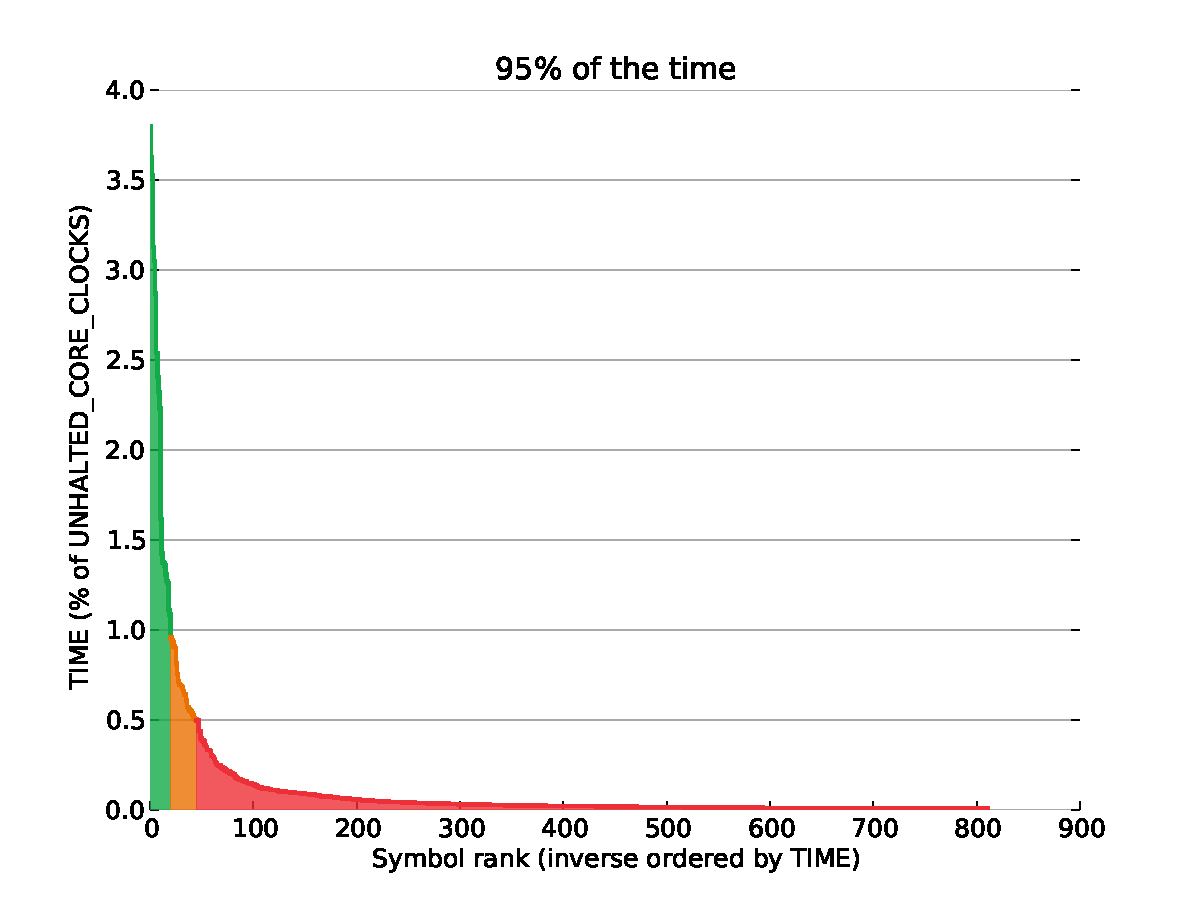
\includegraphics{unhalted_core_clock-series2.pdf}}
\end{center}
\end{figure}



As it can be seen from the plot the aggregate cost of all the methods using less than 0.5\% of the total time sums up to 44\% of the total cost. Due do the small per symbol cost we need an high resolution tool for doing the profile and that's why perfmon2 becomes attractive for a proper analysis.


In order to understand how to proceed for symbols found in the tail of the distribution we decided to join timing information with those coming from some other processor counter. This way we correlate cost with its possible cause and it's therefore easier to look at the source and take a specific action. If for example we plot the counts for \texttt{CLOCK\_CORE\_UNHALTED} and \texttt{ITLB\_MISS\_RETIRED} together, using the former to order symbols in both cases.


\begin{figure}
\caption{}
\label{}
\begin{center}
\resizebox{250pt}{!}{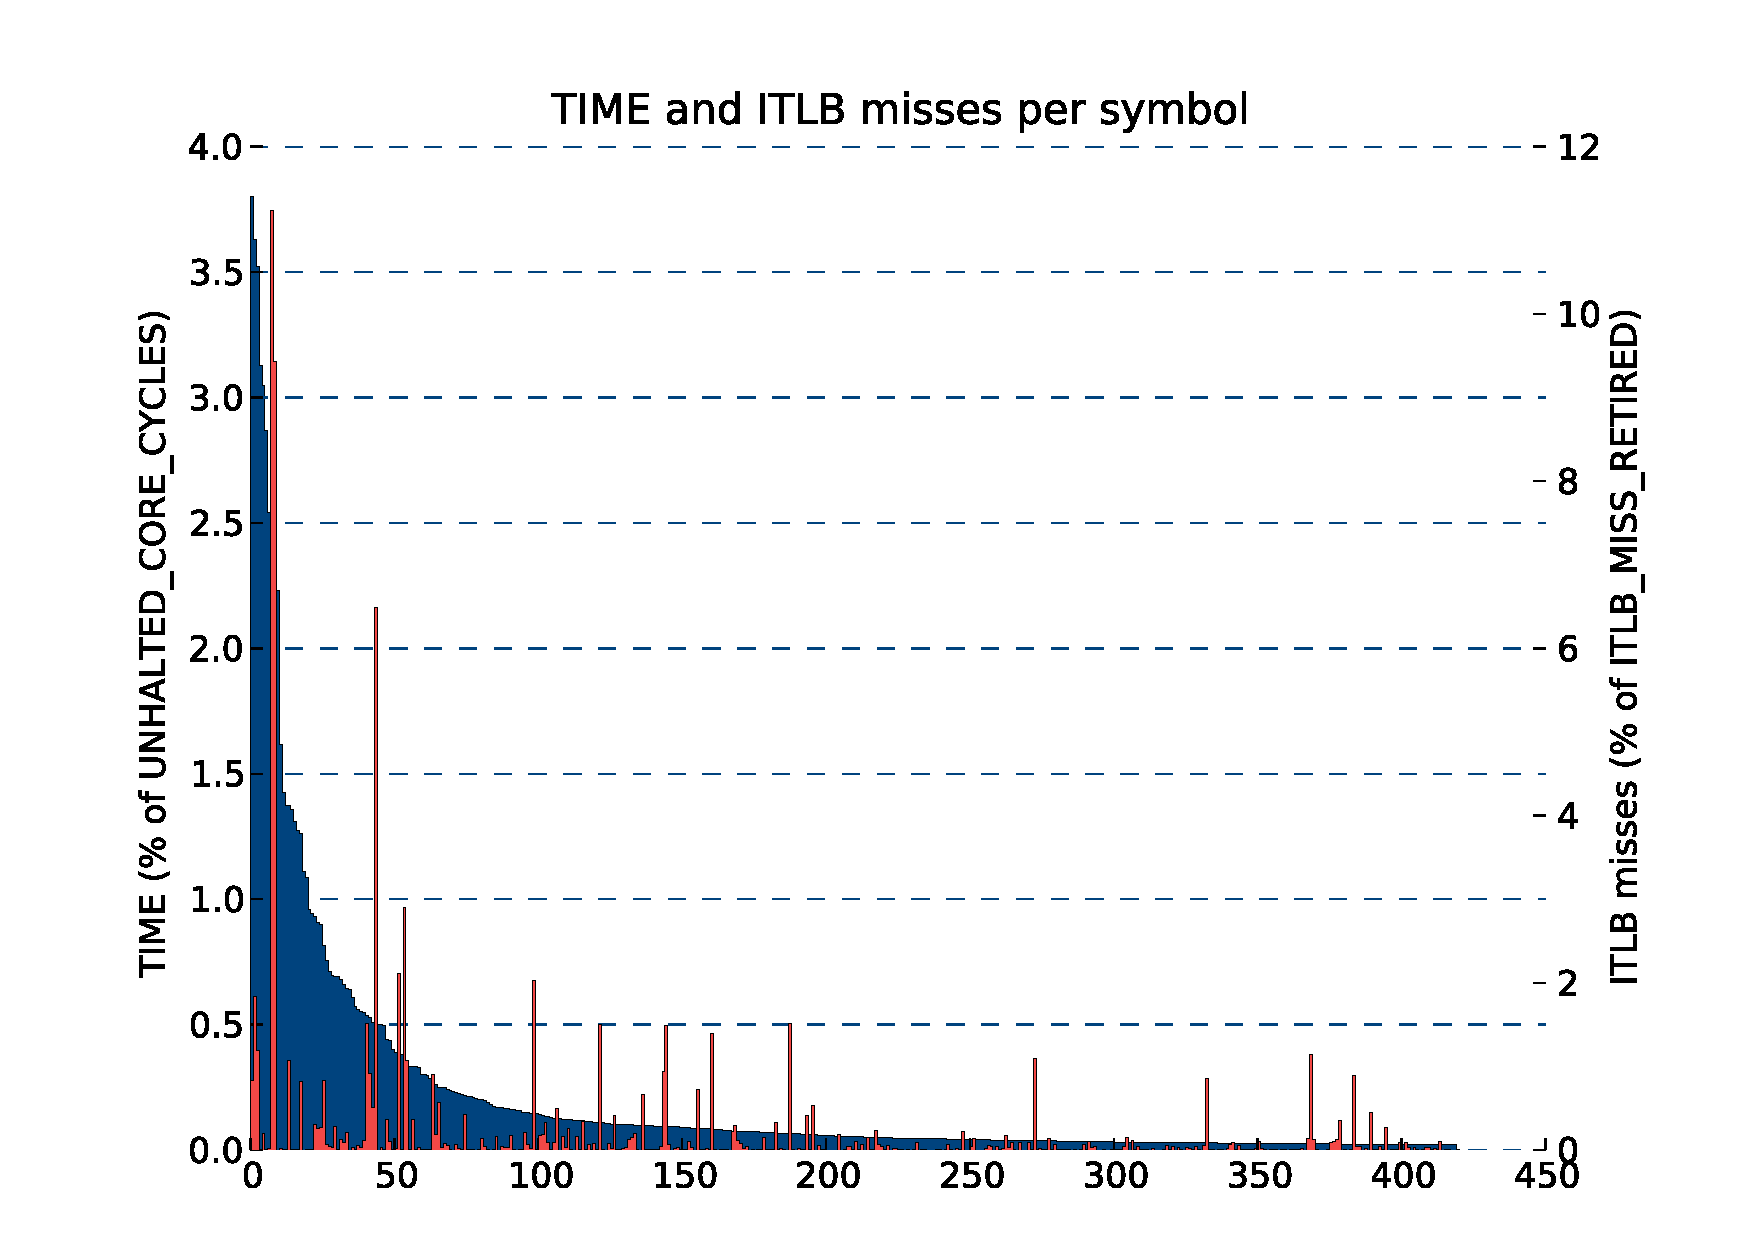
\includegraphics{correlation-plot.pdf}}
\end{center}
\end{figure}



We immediately see that there is not a complete correlation between them and that some symbols suffer more for the \texttt{ITLB\_MISS\_RETIRED} than others. Similar information can be obtained doing a scatter plot, where each marker in the plot is a given symbol in the code.


\begin{figure}
\caption{}
\label{}
\begin{center}
\resizebox{250pt}{!}{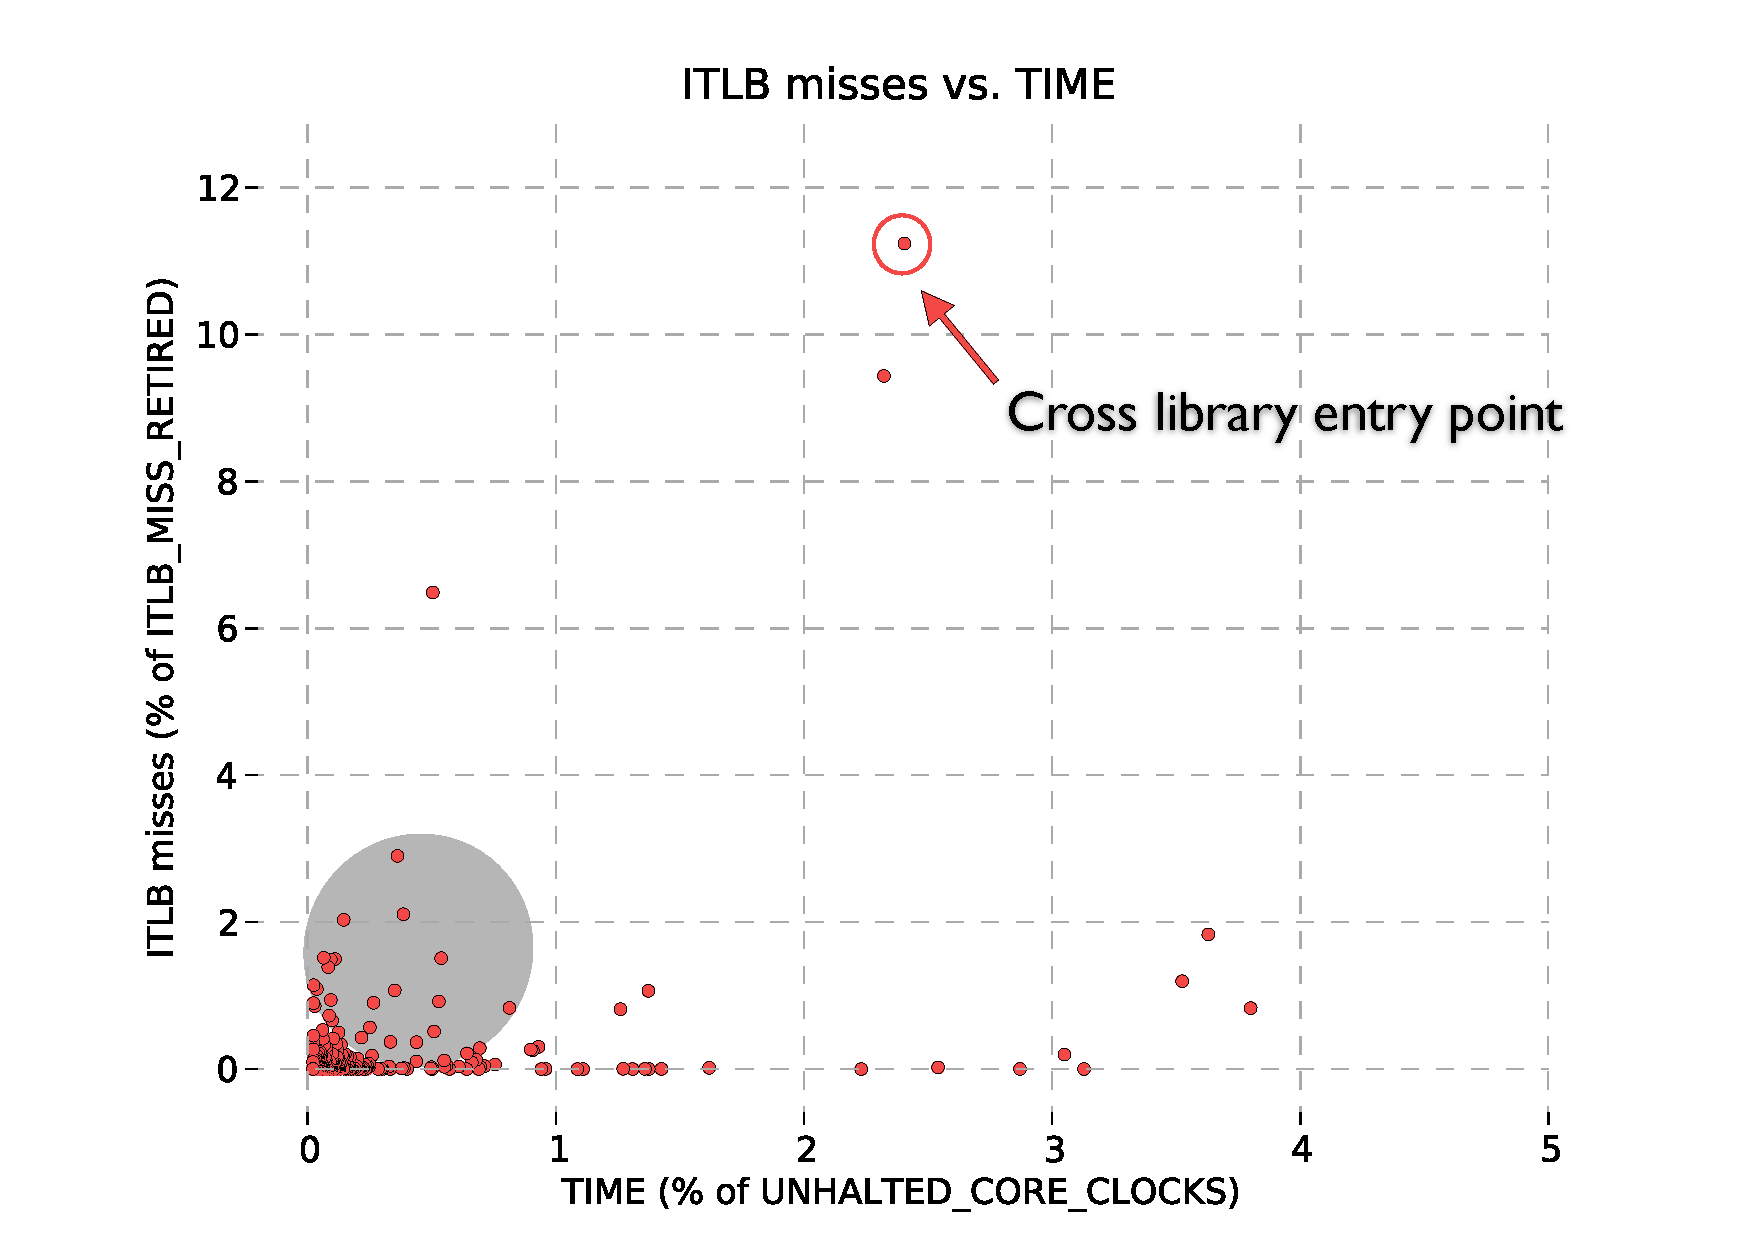
\includegraphics{scatter-plot.pdf}}
\end{center}
\end{figure}



Here for example we see again that the inter-library entry point suffers a lot because of ITLB misses, as we would expect. However, as we said, this has to be (and is being) addressed with a global redisign of the way we package our software, which will take time and agreement between the various parties involved.
What has a more limited impact but is also more immediate to address and fix are the problems with symbols in the {\itshape grey area}. They still show up in the reports with relatively a measurable amount of time (between 0.3\% and 0.5\%) and most important show a significant footprint (few percents) due to some specific problem (ITLB misses in this case). Moreover, as we have previously said this code is most likely coming from the truly physics related part of the software and therefore under stricter control and most likely with limited scope.


\subsection{Case study}
\label{casestudy}

One particular example we have found in our investigation indeed comes from an analysis on our software like the one suggested. The problem was insulated to be in the constructor of one of the classes representing a symmetric matrix. What was happening in this case was due to a static variable local to the constructor of the class being used to initialize a lookup table needed to speed up the serialization of objects of that class. An analysis of produced code revealed that the compiler we used (\texttt{gcc} 3.4.5) was unable to detect the code as a one time initialization and to move it out of the constructor itself. An otherwise trivial constructor was therefore carrying along the full code for a one time initialisation of a lookup table. We think this hidden cost was effectively creating problems in two ways:


\begin{itemize}


\item the code for the symbol was too large to be inlined efficiently and was in general fooling the inline heuristics for that particular bit of code.

\item the initialization code, albeit not being executed, still had influnce on the pressure on the ITLB and instruction cache.
\end{itemize}

Changing the constructor forcing the time initialisation code to be out-of-line had the expected result of reducing the size of the symbol for the constructor from 300 bytes to 30. Moreover, accurate measurements on the performance of the global software not only showed a 0.3\% improvement in the total execution time, but they also showed that the the improvement in performance itself was concentrated in those symbols which referred to the above mentioned matrix class in their signature (7\% improvement for those).


\begin{figure}
\caption{}
\label{}
\begin{center}
\resizebox{350pt}{!}{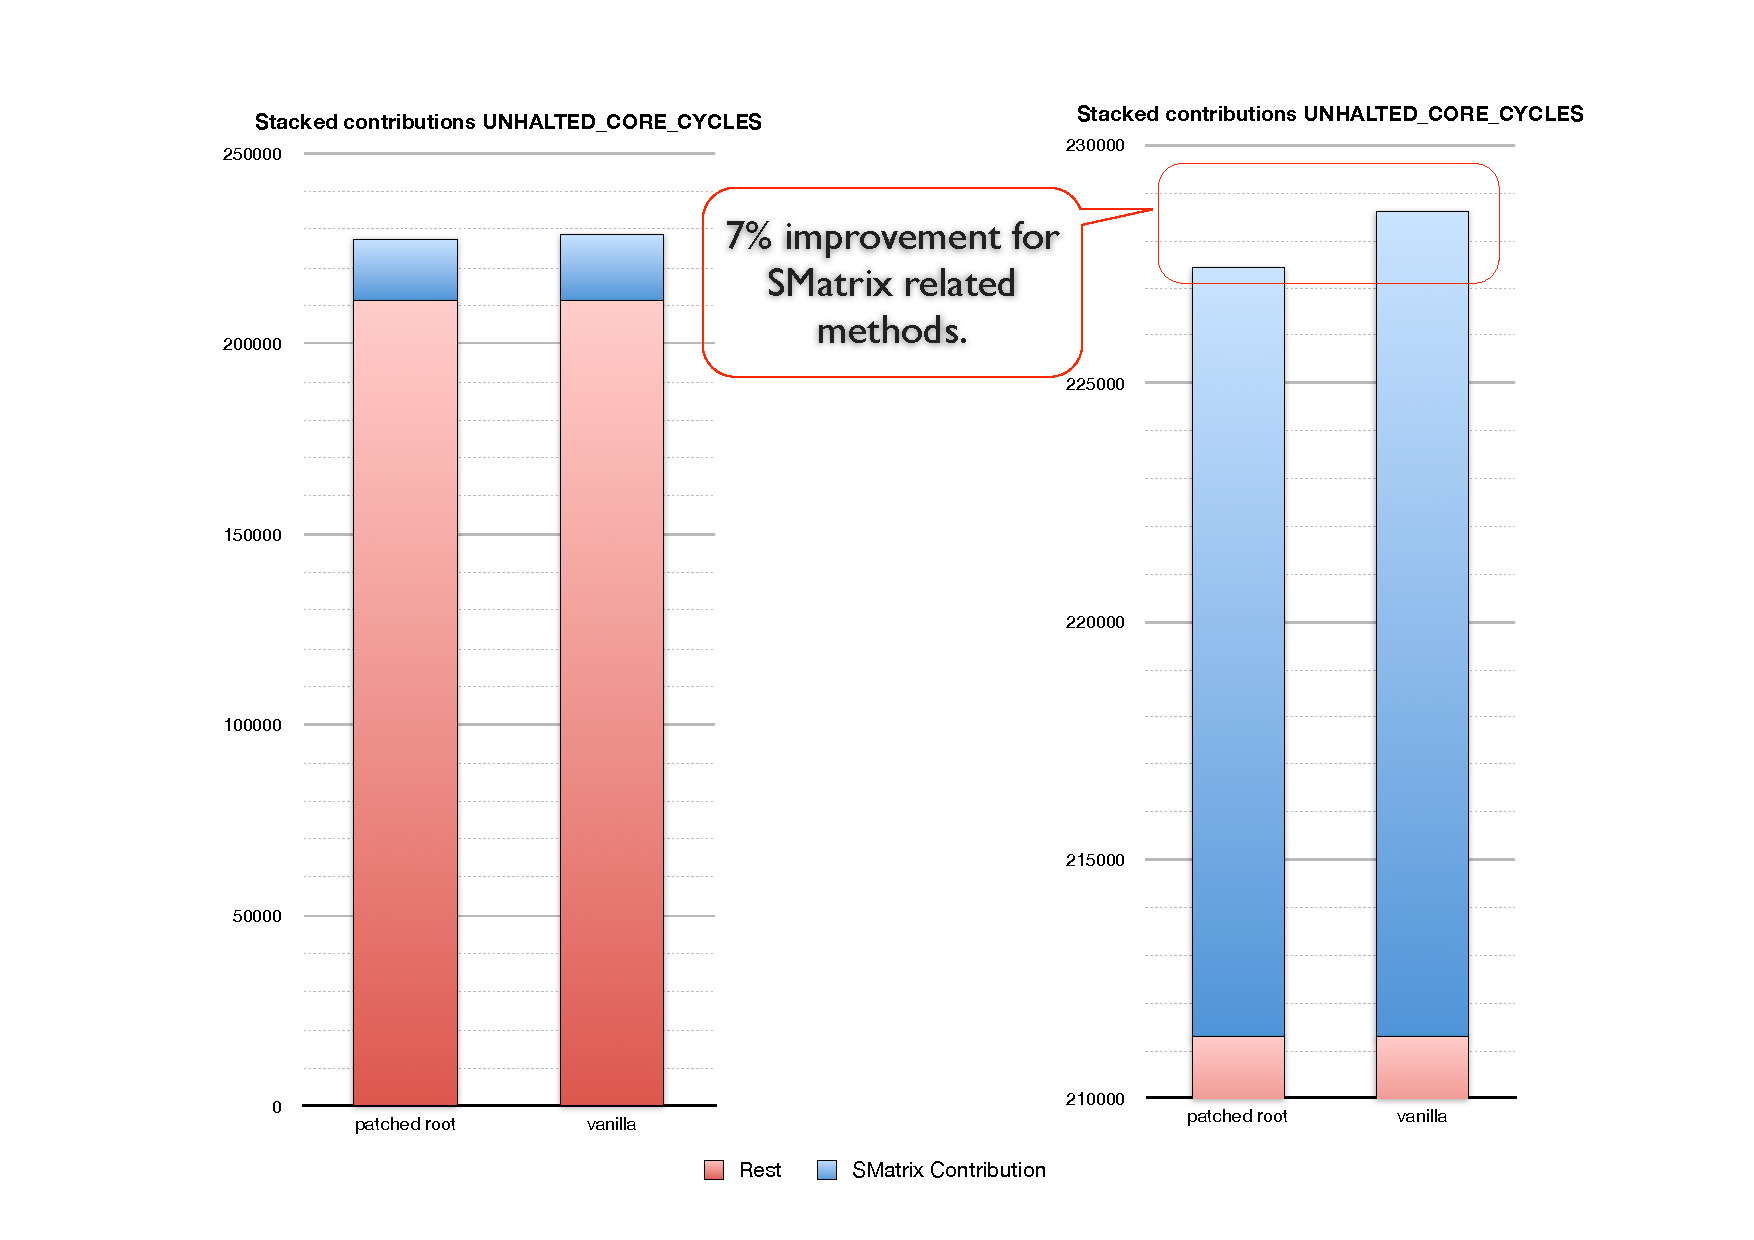
\includegraphics{smatrix-improvement.pdf}}
\end{center}
\end{figure}



We were also encouraged by the fact that a more recent version of the compiler (\texttt{gcc} 4.3.2) did autonomously exactly the same thing. While 0.3\% of the execution time might be seen as a minor improvement one must think that one has to factor out the initial part of the distribution (which as we said is due to dynamic memory usage) and moreover it's important to note that due to the nature of the time distribution is not possible to expect anything much better from a single improvement.


\section{Conclusions}
\label{conclusions}

In the last year we have successfully profited from the experience and tools to profiling our software developed within CMS over the time (~\cite{Tuura:2008p00019}, ~\cite{Elmer:2009}, ~\cite{Eulisse:2004}, ~\cite{Eulisse:2004igprof}). We have confirmed to ourselves that the methodology discussed in the past ~\cite{Tuura:2008p00019} is indeed useful and we have extended it to include symbol size analysis and code coverage information. We have improved our understanding of compiler code generation and we have been able to exploit this knowledge to address several code bloat issues present in our code. Moreover we have have also developed a new methodology on how to use perfmon2 profiling results to obtain precise information about where and how to intervene on the code and we plan to further develop this methodology as it looks promising to guide optimization efforts.


\section{Aknowledgements}
\label{aknowledgements}

For the support, space and contributions to discussion we would like to thank the rest of CMS Offline Software Group, the CERN MultiCore R\&D group and in particular Vincenzo Innocente. For the support given both in terms of hardware and software configuration we would like to thank the CERN PH/SFT division, the Estonian National Institute of Chemical Physics and Biophysics (NICPB), and in particular Stefan Roiser, Gilles Raymond (CERN), Mario Kadastik and Ilja Livenson (NICPB). Finally a special thanks goes to Stephan Eranian (ex HP, now at Google Inc.) for the excellent work he did on the perfmon2 profiler. This work would also have never been possible without support of the National Science Foundation of the United States of America.


\section{References}
\label{references}

\begin{thebibliography}{0}


\bibitem{Moore:1998p325}
Moore, G. (1998). Cramming more components onto integrated circuits. {\itshape Proceedings of the IEEE}.

\bibitem{Smith:1998}
Smith. A study of branch prediction strategies. {\itshape International Symposium on Computer Architecture.} (1998)

\bibitem{Uht:1997}
Uht, A. K., Sindagi, V., \& Somanathan, S. (1997). Branch effect reduction techniques. Computer, 30(5), 71-81.

\bibitem{Core2Duo}
http://www.intel.com

\bibitem{Innocente:2009}
Innocente, V. (2009). The challenge of adapting HEP physics software applications to run on many-core cpus. {\itshape Proceedings of Computing in High-Energy and Nuclear Physics (CHEP09)}, Prague, 2009.

\bibitem{Jones:2006}
C. Jones et al. The new CMS Event Data Model and Framework. {\itshape Proceedings of Computing in High-Energy and Nuclear Physics (CHEP06)}, Mumbai, 2006.

\bibitem{Elmer:2009}
Elmer, P., Eulisse, G., Tuura, L. A., Innocente, V. (2009). {\itshape Proceedings of Computing in High-Energy and Nuclear Physics (CHEP09)}, Prague, 2009.

\bibitem{Tuura:2008p00019}
Tuura, L., Innocente, V., \& Eulisse, G. (2008). Analysing CMS software performance using IgProf, OProfile and callgrind. {\itshape J. Phys.: Conf. Ser.} 119 Volume 119 042030 (8pp).

\bibitem{Eranian:2006p467}
Eranian, S. (2006) Perfmon2: a flexible performance monitoring interface for Linux. {\itshape Proc. of the 2006 Ottawa Linux Symposium}, Ottawa, 2006.

\bibitem{Anderson:1997}
Anderson et al. (1997) Continuous profiling: Where have all the cycles gone? {\itshape ACM Transactions on Computer Systems TOCS}.

\bibitem{Eulisse:2004igprof}
Eulisse, G., \& Tuura, L. (2004) IgProf profiling tool.
{\itshape Proceedings of Computing in High-Energy and Nuclear Physics (CHEP04)}, Interlaken, 2004.

\bibitem{Eulisse:2004}
Eulisse, G., Muzaffar, S., Osborne, I., Taylor, L., \& Tuura, L. A. (2004). A coherent environment of software improvement tools for CMS. {\itshape Nuclear Inst. and Methods in Physics Research}, 534, 138-142.
		
\end{thebibliography}
		
%
% Back Matter
%

%	Bibliography
\bibliographystyle{\mybibliostyle}
\bibliocommand

\end{document}
